\documentclass[a4paper,10pt]{article} % na razie jako article, jak będzie więcej treści zmieni się na report.

\usepackage[polish]{babel}
\usepackage[utf8]{inputenc}
\usepackage{polski}
\usepackage[T1]{fontenc}

\usepackage{indentfirst}
\usepackage{amsmath, amstext} % ,amsfonts,amssymb
\usepackage{verbatim}
\usepackage{booktabs}
\usepackage{color}
\usepackage[usenames,dvipsnames,svgnames]{xcolor}
\usepackage{utopia}
\usepackage{geometry}
\geometry{verbose,lmargin=3cm,rmargin=3cm}
\frenchspacing

\usepackage{graphicx}

% podtytuł
\usepackage{titling}
\newcommand{\subtitle}[1]{
 \posttitle{
  \par\end{center}
  \begin{center}\large#1\end{center}
  \vskip0.5em}
}

%opening
\title{Nowe Trendy w Obliczeniach Neuronowych}
\subtitle{Spike and Slab Restricted Boltzmann Machine w klasyfikacji obiektów ze zbioru CIFAR-10}
\author{Konrad Brus \\ Jakub A. Gramsz}

\begin{document}
\maketitle

\begin{abstract}
Projekt ma na celu implementację Gaussian Restricted Boltzmann Machine oraz Spike and Slab RBM (zaprezentowanych w \cite{courville2013spike}) i wykorzystanie ich do klasyfikacji obiektów przedstawionych na obrazach. Implementacja uczona oraz testowana będzie na zbiorze danych CIFAR-10 (przedstawiony w \cite{cifar}) przy wykorzystaniu algorytmu uczenia Contrastive Divergence.
\end{abstract}

\section{Wstęp teoretyczny}
Maszyna Boltzmanna (ang. \textit{Boltzmann Machine}, BM) jest nieskierowanym grafem probabilistycznym z
węzłami o wartościach dyskretnych lub ciągłych. Model BM można interpretować jako stochastyczną sieć
neuronową, w której stan każdego neuronu zależy od neuronów do niego połączonych. Początkowo
zaproponowano maszynę Boltzmanna jako graf pełny z neuronami o wartościach binarnych, taka sieć była
analogiczna do sieci Hopfielda jeżeli zastosowalibyśmy neurony deterministyczne zamiast stochastycznych.
Zaletą maszyny Boltzmanna nad siecią Hopfielda jest, to że maszyna Boltzmanna potrafi generować próbki
na podstawie wyuczonego rozkładu prowdopodobieństwa.

\begin{figure}
 \centering
 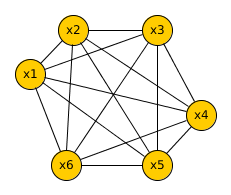
\includegraphics[width=5cm]{imgs/bm.png}
 \label{fig:bm}
\caption{Maszyna Boltzmanna, wszystkie neurony są połączone ze wszystkimi}
\end{figure} 

Szybko zauważono, że utrzymywanie wszystkich połączeń w maszynie Boltzmanna przynosi negatywne skutki.
Uczenie takiego modelu było bardzo trudne i długotrwałe, a jakość wyników nie była wystarczająco dobra
(jak na taki czas generowania modelu). Ograniczono, więc liczbę połączeń w sieci, wierzchołki podzielono
na dwie grupy warstwę widoczną i warstwę ukrytą. W nowym modelu ograniczonej maszynie Boltzmanna (ang.
\textit{Restricted Boltzmann Machine}) usunięto wszystkie połączenia pomiędzy neuronami tej samej
warstwy.

\begin{figure}
 \centering
 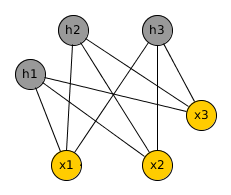
\includegraphics[width=5cm]{imgs/rbm.png}
 \label{fig:rbm}
\caption{Ograniczona maszyna Boltzmanna, połączenia występują pomiędzy wyszystkimi neuronami z różnych
warstw}
\end{figure} 

\section{Opis problemu}

Rozpatrywany problem można uznać za problem klasyfikacji, a więc zastosowany model można uznać ze typ klasyfikatora. Na jego wejście podawany jest, w postaci mapy bitowej, obraz należący do jednej z klas, na wyjściu zaś pojawia się etykieta klasy. Aby tego dokonać zestawiane są dwie ograniczone maszyny Boltzmanna, z których pierwsza służy do ekstrakcji cech z danych wejściowych, a druga przydziela tak otrzymane cechy do jednej z 10 klas.

\section{Opis modelu}

Najbardziej podstawową wersją ograniczonej maszyny Boltzmanna jest odmiana BB-RBM (Binary-Binary RBM). Składa się ona z warstwy binarnych jednostek widocznych oraz binarnych jednostek ukrytych, co wymusza binarną reprezentację danych wejściowych $x$ i skutkuje binarną reprezentacją ukrytą $h$.

W takiej formie, każda jednostka widoczna $x_i$ oraz ukryta $h_j$ posiadają wejścia bias \textit{$b_i$} oraz \textit{$c_j$}. Jednostka ukryta z widoczną połączone są wagami \textit{$w_ij$}.

Dla modelu RBM definuje się funkcję energii \textbf{E}, określoną:

\begin{align}
	\mathbf{E_{BB-RBM}(x,h) = -x^Tb - c^Th - x^TWh}
\end{align}

Nie jest to najbardziej intuicyjne podejście w przypadku modelowania obrazów (i, w ogólności, danych pochodzących z dziedziny rzeczywistej), co umotywowało utworzenie wersji RBM, w której warstwa ukryta jest w dalszym ciągu binarna, lecz warstwa widoczna jest ciągła i ma rozkład normalny o średniej $b_i$ i wariancji $\sigma^2_i$. Odmiana taka to GB-RBM (Gaussian-Binary RBM).

Z taką odmianą skojarzona jest następująca funkcja energii:

\begin{align}
	\mathbf{E_{GB-RBM}(x,h) = \left\| \frac{x - b}{2 \sigma} \right\| ^2 - c^Th - \left( \frac{x}{\sigma^2} \right) ^TWh}
\end{align}

\section{Opis algorytmu uczenia}

\section{Opis eksperymentu i  zbioru danych}
Do badań zostanie użyty zbiór CIFAR-10. Zawiera on 60000 kolorowych obrazów o wymiarach 32x32 pikseli, należących do jednej z 10 klas: 
\begin{itemize}
	\item airplane, automobile, bird \\
	\begin{center} 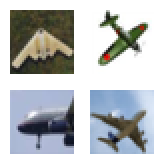
\includegraphics{imgs/class_0.png} 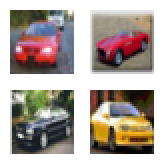
\includegraphics{imgs/class_1.png} 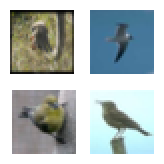
\includegraphics{imgs/class_2.png} \end{center}

	\item cat, deer, dog \\
	\begin{center} 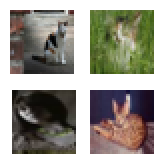
\includegraphics{imgs/class_3.png} 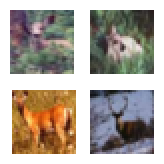
\includegraphics{imgs/class_4.png} 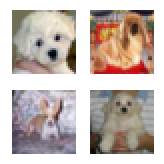
\includegraphics{imgs/class_5.png} \end{center}

	\item frog, horse, ship \\
	\begin{center} 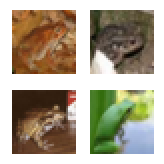
\includegraphics{imgs/class_6.png} 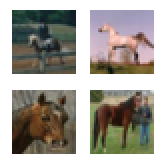
\includegraphics{imgs/class_7.png} 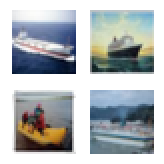
\includegraphics{imgs/class_8.png} \end{center}

	\item truck \\
	\begin{center} 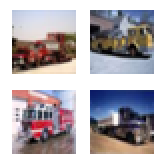
\includegraphics{imgs/class_9.png} \end{center}
\end{itemize}

Na jedną klasę przypada 6000 obrazów.

Zbiór jest wstęnie podzielony na dwie części - treningową (zawierającą 50000 obrazów, 5000 na klasę) oraz walidacyjną (10000 obrazów, 1000 na klasę).

\section{Dostrajanie modelu i wyniki}

\section{Dyskusja i wnioski}


\bibliographystyle{abbrv}
\nocite{*} % na razie póki mało co jest cytowane (powoduje że wszystko z listy artykułów jest tu widoczne
\bibliography{lit}

\end{document}
